\documentclass[12pt]{article}
\usepackage[left=1cm, right=1cm, top=2cm,bottom=1.5cm]{geometry} 

\usepackage[parfill]{parskip}
\usepackage[utf8]{inputenc}
\usepackage[T2A]{fontenc}
\usepackage[russian]{babel}
\usepackage{enumitem}
\usepackage[normalem]{ulem}
\usepackage{amsfonts, amsmath, amsthm, amssymb, mathtools,xcolor,accents}
\usepackage{blkarray}

\usepackage{tabularx}
\usepackage{hhline}

\usepackage{accents}
\usepackage{fancyhdr}
\pagestyle{fancy}
\renewcommand{\headrulewidth}{1.5pt}
\renewcommand{\footrulewidth}{1pt}

\usepackage{graphicx}
\usepackage[figurename=Рис.]{caption}
\usepackage{subcaption}
\usepackage{float}

%%Наименование папки откуда забирать изображения
\graphicspath{ {./images/} }

%%Изменение формата для ввода доказательства
\renewcommand{\proofname}{$\square$  \nopunct}
\renewcommand\qedsymbol{$\blacksquare$}

%%Изменение отступа на таблицах
\addto\captionsrussian{%
	\renewcommand{\proofname}{$\square$ \nopunct}%
}
%% Римские цифры
\newcommand{\RN}[1]{%
	\textup{\uppercase\expandafter{\romannumeral#1}}%
}

%% Для удобства записи
\newcommand{\MR}{\mathbb{R}}
\newcommand{\MC}{\mathbb{C}}
\newcommand{\MQ}{\mathbb{Q}}
\newcommand{\MN}{\mathbb{N}}
\newcommand{\MZ}{\mathbb{Z}}
\newcommand{\MTB}{\mathbb{T}}
\newcommand{\MTI}{\mathbb{I}}
\newcommand{\MI}{\mathrm{I}}
\newcommand{\MCI}{\mathcal{I}}
\newcommand{\MJ}{\mathrm{J}}
\newcommand{\MH}{\mathrm{H}}
\newcommand{\MT}{\mathrm{T}}
\newcommand{\MU}{\mathcal{U}}
\newcommand{\MV}{\mathcal{V}}
\newcommand{\MB}{\mathcal{B}}
\newcommand{\MF}{\mathcal{F}}
\newcommand{\MW}{\mathcal{W}}
\newcommand{\ML}{\mathcal{L}}
\newcommand{\MP}{\mathcal{P}}
\newcommand{\VN}{\varnothing}
\newcommand{\VE}{\varepsilon}
\newcommand{\dx}{\, dx}
\newcommand{\dy}{\, dy}
\newcommand{\dz}{\, dz}
\newcommand{\dd}{\, d}


\theoremstyle{definition}
\newtheorem{defn}{Опр:}
\newtheorem{rem}{Rm:}
\newtheorem{prop}{Утв.}
\newtheorem{exrc}{Упр.}
\newtheorem{problem}{Задача}
\newtheorem{lemma}{Лемма}
\newtheorem{theorem}{Теорема}
\newtheorem{corollary}{Следствие}

\newenvironment{cusdefn}[1]
{\renewcommand\thedefn{#1}\defn}
{\enddefn}

\DeclareRobustCommand{\divby}{%
	\mathrel{\text{\vbox{\baselineskip.65ex\lineskiplimit0pt\hbox{.}\hbox{.}\hbox{.}}}}%
}
\DeclareRobustCommand{\ndivby}{\mkern-1mu\not\mathrel{\mkern4.5mu\divby}\mkern1mu}


%Короткий минус
\DeclareMathSymbol{\SMN}{\mathbin}{AMSa}{"39}
%Длинная шапка
\newcommand{\overbar}[1]{\mkern 1.5mu\overline{\mkern-1.5mu#1\mkern-1.5mu}\mkern 1.5mu}
%Функция знака
\DeclareMathOperator{\sgn}{sgn}

%Функция ранга
\DeclareMathOperator{\rk}{\text{rk}}
\DeclareMathOperator{\diam}{\text{diam}}


%Обозначение константы
\DeclareMathOperator{\const}{\text{const}}

\DeclareMathOperator{\codim}{\text{codim}}

\DeclareMathOperator*{\dsum}{\displaystyle\sum}
\newcommand{\ddsum}[2]{\displaystyle\sum\limits_{#1}^{#2}}
\newcommand{\ddssum}[2]{\displaystyle\smashoperator{\sum\limits_{#1}^{#2}}}
\newcommand{\ddlsum}[2]{\displaystyle\smashoperator[l]{\sum\limits_{#1}^{#2}}}
\newcommand{\ddrsum}[2]{\displaystyle\smashoperator[r]{\sum\limits_{#1}^{#2}}}

%Интеграл в большом формате
\DeclareMathOperator{\dint}{\displaystyle\int}
\newcommand{\ddint}[2]{\displaystyle\int\limits_{#1}^{#2}}
\newcommand{\ssum}[1]{\displaystyle \sum\limits_{n=1}^{\infty}{#1}_n}

\newcommand{\smallerrel}[1]{\mathrel{\mathpalette\smallerrelaux{#1}}}
\newcommand{\smallerrelaux}[2]{\raisebox{.1ex}{\scalebox{.75}{$#1#2$}}}

\newcommand{\smallin}{\smallerrel{\in}}
\newcommand{\smallnotin}{\smallerrel{\notin}}

\newcommand*{\medcap}{\mathbin{\scalebox{1.25}{\ensuremath{\cap}}}}%
\newcommand*{\medcup}{\mathbin{\scalebox{1.25}{\ensuremath{\cup}}}}%

\makeatletter
\newcommand{\vast}{\bBigg@{3.5}}
\newcommand{\Vast}{\bBigg@{5}}
\makeatother

%Промежуточное значение для sup\inf, поскольку они имеют разную высоту
\newcommand{\newsup}{\mathop{\smash{\mathrm{sup}}}}
\newcommand{\newinf}{\mathop{\mathrm{inf}\vphantom{\mathrm{sup}}}}

%Скалярное произведение
\newcommand{\inner}[2]{\left\langle #1, #2 \right\rangle }
\newcommand{\linsp}[1]{\left\langle #1 \right\rangle }
\newcommand{\linmer}[2]{\left\langle #1 \vert #2\right\rangle }

%Подпись символов снизу
\newcommand{\ubar}[1]{\underaccent{\bar}{#1}}

%%Шапка для букв сверху
\newcommand{\wte}[1]{\widetilde{#1}}
\newcommand{\wht}[1]{\widehat{#1}}
\newcommand{\ovl}[1]{\overline{#1}}


%%Трансформация Фурье
\newcommand{\fourt}[1]{\mathcal{F}\left(#1\right)}
\newcommand{\ifourt}[1]{\mathcal{F}^{-1}\left(#1\right)}

%%Символ вектора
\newcommand{\vecm}[1]{\overrightarrow{#1\,}}

%%Пространстов матриц
\newcommand{\matsq}[1]{\operatorname{Mat}_{#1}}
\newcommand{\mat}[2]{\operatorname{Mat}_{#1, #2}}

%Оператор для действ и мнимых чисел
\DeclareMathOperator{\IM}{\operatorname{Im}}
\DeclareMathOperator{\RE}{\operatorname{Re}}
\DeclareMathOperator{\li}{\operatorname{li}}
\DeclareMathOperator{\GL}{\operatorname{GL}}
\DeclareMathOperator{\SL}{\operatorname{SL}}
\DeclareMathOperator{\Char}{\operatorname{char}}
\DeclareMathOperator\Arg{Arg}
\DeclareMathOperator\ord{ord}

%Оператор для образа
\DeclareMathOperator{\Ima}{Im}

%Делимость чисел
\newcommand{\modn}[3]{#1 \equiv #2 \; (\bmod \; #3)}
\newcommand{\nmodn}[3]{#1 \not\equiv #2 \; (\bmod \; #3)}

%%Взятие в скобки, модули и норму
\newcommand{\parfit}[1]{\left( #1 \right)}
\newcommand{\modfit}[1]{\left| #1 \right|}
\newcommand{\sqparfit}[1]{\left\{ #1 \right\}}
\newcommand{\normfit}[1]{\left\| #1 \right\|}

%%Функция для обозначения равномерной сходимости по множеству
\newcommand{\uconv}[1]{\overset{#1}{\rightrightarrows}}
\newcommand{\uconvm}[2]{\overset{#1}{\underset{#2}{\rightrightarrows}}}

%% Функция для добавления круга сверху множества
\newcommand{\Circ}[1]{\accentset{\circ}{#1}}

%%Функция для обозначения нижнего и верхнего интегралов
\def\upint{\mathchoice%
	{\mkern13mu\overline{\vphantom{\intop}\mkern7mu}\mkern-20mu}%
	{\mkern7mu\overline{\vphantom{\intop}\mkern7mu}\mkern-14mu}%
	{\mkern7mu\overline{\vphantom{\intop}\mkern7mu}\mkern-14mu}%
	{\mkern7mu\overline{\vphantom{\intop}\mkern7mu}\mkern-14mu}%
	\int}
\def\lowint{\mkern3mu\underline{\vphantom{\intop}\mkern7mu}\mkern-10mu\int}

%%След матрицы
\DeclareMathOperator*{\tr}{tr}

\makeatletter
\renewcommand*\env@matrix[1][*\c@MaxMatrixCols c]{%
	\hskip -\arraycolsep
	\let\@ifnextchar\new@ifnextchar
	\array{#1}}
\makeatother


%% Переопределение функции хи, чтобы выглядела более приятно
\makeatletter
\@ifdefinable\@latex@chi{\let\@latex@chi\chi}
\renewcommand*\chi{{\@latex@chi\smash[t]{\mathstrut}}} % want only bottom half of \mathstrut
\makeatletter

\setcounter{MaxMatrixCols}{20}

\begin{document}
\lhead{Математический анализ - \RN{4}}
\chead{Шапошников С.В.}
\rhead{Лекция - 4}

\section*{Критерий Лебега}
\begin{theorem}(\textbf{Критерий Лебега})
	$f$ интегрируема по Риману на $\MI \Leftrightarrow f$ - ограничена и $f$ - непрерывна почти всюду на $\MI$.
\end{theorem}
\begin{rem}
	Заметим, что доказать эту теорему можно идентично тому, что было во $2$-м семестре (см. лекцию $25$). Сейчас же мы докажем теорему немного по-другому, использовав факт, который станит понятен только в дальнейшем, но позволяющий доказать эту теорему проще.
\end{rem}
\begin{proof}
	Предполагаем, что $f$ - ограниченна. По критерию интегрируемости, пусть у нас есть $\{\MI_m^N\}$ - разбиение бруска $\MI$ на попарно непересекающиеся бруски так, что $\diam(\MI_m^N) < \tfrac{1}{N}$ и $N+1$-ое разбиение получается из $N$-го разбиением уже имеющихся брусков. Для таких разбиений мы определяли две функции:
	$$
		h_N(x) = \ddsum{m}{}\inf\limits_{\MI_m^N}f(x){\cdot}\chi_{\MI_m^N}(x), \quad g_N(x) = \ddsum{m}{}\sup\limits_{\MI_m^N}f(x){\cdot}\chi_{\MI_m^N}(x)
	$$
	Тогда по критерию интегрируемости верно:
	$$
		f \text{ - интегрируема на } \MI \Leftrightarrow \ddint{\MI}{}(\underbrace{g_N(x) - h_N(x)}_{\geq 0})dx \xrightarrow[N \to \infty]{} 0
	$$
	Рассмотрим внимательнее подинтегральное выражение:
	$$
		g_N(x) - h_N(x) = \ddsum{m}{}(\sup\limits_{\MI_m^N}f(x) - \inf\limits_{\MI_m^N}f(x)){\cdot}\chi_{\MI_m^N}(x) = \ddsum{m}{}\omega(f,\MI_m^N){\cdot}\chi_{\MI_m^N}(x)
	$$
	Возьмем $x \in \MI$ такой, что $x$ не принадлежит границам $\MI_m^N, \, \forall m,N$, то есть каждый раз эта точка оказывается внутри бруска разбиения. Возьмем $\delta > 0$ и рассмотрим шар $\MB(x,\delta) \Rightarrow$ брус содержащий $x$ попадет в шар $\MB(x,\delta)$ с ростом $N \Rightarrow$ колебание на брусе будет меньше, чем на шаре:
	$$
		\diam(\MI_m^N) < \dfrac{1}{N} \to 0 \Rightarrow \exists \, N \colon \MI_m^N \subset \MB(x,\delta) \Rightarrow \omega(f,\MI_m^N) \leq \omega(f,\MB(x,\delta))
	$$
	где последнее верно, в силу того, что при расширении множества $\sup$ может только возрасти,а $\inf$ только уменьшиться (см. лекцию $2$ этого семестра). Вспомним, что колебание в точке $\omega_f(x)$ это предел:
	$$
		\omega_f(x) = \lim\limits_{\delta \to 0+}\omega(f,\MB(x,\delta))
	$$
	Про это можно посмотреть, в лекции $17$ семестра $1$ и лекции $25$ семестра $2$. Возьмем $\VE > 0$, тогда: 
	$$
		\exists \, \delta > 0 \colon \omega(f,\MB(x,\delta)) < \omega_f(x) + \VE \Rightarrow \omega(f,\MI_m^N) < \omega_f(x) + \VE \Rightarrow g_N(x) - h_N(x) < \omega_f(x) + \VE
	$$
	где последнее верно в силу того, что: $x \in \MI_m^N \Rightarrow \chi_{\MI_m^N}(x) = 1, \, \forall k \neq m, \, \chi_{\MI_k^N}(x) = 0$. Таким образом:
	$$
		\forall \VE > 0, \, \exists \, N_0 \colon \forall N > N_0, \, g_N(x) - h_N(x) < \omega_f(x) + \VE
	$$
	Точка $x \in \MI_m^N$ не принадлежит граням этого бруска $\Rightarrow$ она внутренняя, тогда:
	$$
		\exists \, \gamma > 0  \colon \MB(x,\gamma) \subset \MI_m^N \Rightarrow \omega(f,\MB(x,\gamma)) \leq \omega(f,\MI_m^N)
	$$
	Когда мы стягиваем шары, то колебания на них не возрастают при уменьшении радиуса, тогда:
	$$
		\omega_f(x) \leq \omega(f,\MB(x,\gamma)) \leq \omega(f,\MI_m^N) \Rightarrow \exists\, N_0 \colon \forall N > N_0, \, \omega_f(x) \leq g_N(x) - h_N(x) \leq \omega_f(x) + \VE
	$$
	Таким образом, для $x$ не принадлежащим граням брусков $\forall m,N, \, \MI_m^N$ мы получаем:
	$$
		g_N(x) - h_N(x) \xrightarrow[N\to  \infty]{} \omega_f(x)
	$$
	Объединение всех граней $\MI_m^N$ по всем $m$ и $N$ является множеством меры нуль по Лебегу, поскольку каждая грань это подмножество $x_k = \const$ - график непрерывной функции над соответствующим параллелепипедом (для конкретного бруска, все его грани это множество меры нуль), а объединение всех граней это объединение счётного набора множеств меры нуль. Тогда:
	$$
		\forall N, \,  |g_N(x) - h_N(x)| \leq 2{\cdot}\sup\limits_{\MI}|f|, \quad g_N(x) - h_N(x) \xrightarrow[N \to \infty]{} \omega_f(x) \text{ п.в. на } \MI \Rightarrow
	$$
	$$
		\Rightarrow \ddint{\MI}{}(g_N(x) - h_N(x))dx \xrightarrow[N\to \infty]{} \ddint{\MI}{}\omega_f(x)dx 
	$$
	где мы пользуемся теоремой Лебега об ограниченной сходимости и утверждением о том, что интеграл Лебега совпадает с интегралом Римана, если функция интегрируема по Риману (мы пока не знакомы с данными утверждениями). Тогда:
	$$
		f \text{ - интегрируема по Риману на } \MI \Leftrightarrow \ddint{\MI}{}\omega_f(x)dx = 0
	$$
	$$	
		\omega_f(x) \geq 0 \Rightarrow \ddint{\MI}{}\omega_f(x)dx = 0 \Leftrightarrow \omega_f(x) = 0 \text{ п.в.}
	$$
	Вспоминая, что: $\omega_f(x) = 0 \Leftrightarrow f$ непрерывна в точке $x$, мы получаем требуемое.
\end{proof}

\begin{corollary}
	Если $f$ интегрируема по Риману на $\MI$, $f \geq 0$ и $\int_\MI f(x)dx = 0$, то $f = 0$ п.в. на $\MI$.
\end{corollary}
\begin{proof}
	Пусть $x_0$ - точка непрерывности функции $f$ и $f(x_0)> 0$, тогда $\exists \, \MJ$ - брусок такой, что:
	$$
		\MJ \subset \MI, \, x_0 \in \MJ, \, |\MJ| > 0, \, f(x) \geq \dfrac{f(x_0)}{2}, \, \forall x \in \MJ
	$$
	Поскольку функция непрерывна и положительна в какой-то точке $\Rightarrow$ в целой окрестности отделена от нуля, окрестность можно взять в виде бруска положительного объема. Тогда можно утверждать:
	$$
		f(x) \geq \dfrac{f(x_0)}{2}{\cdot}\chi_{\MJ}(x) \Rightarrow 0 = \ddint{\MI}{}f(x)dx \geq \ddint{\MI}{}\dfrac{f(x_0)}{2}{\cdot}\chi_\MJ(x)dx = \dfrac{f(x_0)}{2}{\cdot}|\MJ| > 0
	$$
	Получили противоречие $\Rightarrow$ во всех точках непрервности $f = 0 \Rightarrow$ по критерию Лебега $f = 0$ п.в.
\end{proof}
\begin{corollary}
	Если $f$ интегрируема по Риману на $\MI$ и $\varphi$ - непрерывна на $[\inf\limits_\MI f, \sup\limits_\MI f]$, то $\varphi(f)$ интегрируема по Риману на $\MI$.
\end{corollary}
\begin{proof}
	Если функция $\varphi$ непрерывна на $\MI$, то она ограничена на нём $\Rightarrow$ подставили $f$ в ограниченную функцию $\Rightarrow \varphi(f)$ ограничена. Если $f$ непрерывна в $x_0$, то и $\varphi(f)$ непрерывна в $x_0 \Rightarrow \varphi(f)$ непрерывна почти всюду $\Rightarrow \varphi(f)$ по критерию Лебега интегрируема.
\end{proof}
\begin{corollary}
	Если $f$ и $g$ интегрируемы по Риману на $\MI$, то $f{\cdot}g$ интегрируемы на $\MI$.
\end{corollary}
\begin{proof}
	Очевидно, поскольку каждая функция ограничена $\Rightarrow f{\cdot}g$ ограничено. Каждая из них почти всюду непрерывна, но объединение двух множеств меры ноль это множество меры ноль $\Rightarrow$ обе одновременно непрерывны почти всюду, а произведение непрерывных функций - непрерывно $\Rightarrow$ получаем требуемое по критерию Лебега.
\end{proof}

\textbf{Пример}: Рассмотрим функцию Римана и функцию знака:
$$
	R(x) = 
	\begin{cases}
		\dfrac{1}{n}, & x = \dfrac{m}{n}, \, (m,n) = 1 \\
		0, & x \not\in \MQ
	\end{cases}, \quad
	\sgn(x) = 
	\begin{cases}
		1, & x > 0 \\
		0, & x = 0\\
		-1, & x < 0
	\end{cases}
$$
Функция $R(x)$ это ограниченная, почти всюду непрерывная функция $\Rightarrow$ интегрируемая функция. $\sgn(x)$ это интегрируемая функция. Композиция этих функций: $\sgn(R(x)) = D(x)$ это функция Дирихле. Следовательно, композиция функций - не интегрируема.

\begin{rem}
	Пример, когда внутрь подставляем не непрерывную функцию и получаем неинтегрируемую - сложнее. Ранее похожее обсуждалось во $2$-м семестре, когда множество точек разрыва получает положительную меру: используется множество, похожее на Кантаровское, только положительной меры.
\end{rem}

\section*{Интеграл Римана по множеству}
Мы умеем интегрировать только по бруску, но нам хотелось бы научиться интегрировать не только по ним, но и по любому произвольному множеству. 

\textbf{\uline{Идея}}: Пусть у нас есть произвольное множество $A$ и на нём задана функция $f\colon A \to \MR$.  Пусть $A$ это ограниченное множество. Сделаем продолжение функции $f$ на брус $\MI$, содержащий $A$:
$$
	\wte{f}(x) = 
	\begin{cases}
		f(x), & x \in A \\
		0, & x \not\in A
	\end{cases}
$$
\begin{figure}[H]
	\centering
	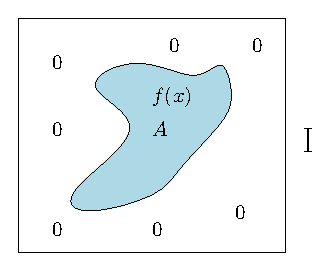
\includegraphics[width=0.25\textwidth]{MA4L4_1.eps}
	\caption{Продолжение функции $f$ на брус $\MI$.}
	\label{4_1}
\end{figure}
Тогда интеграл по множеству $A$ будет иметь вид:
$$
	\ddint{A}{}f(x)dx = \ddint{\MI}{}\wte{f}(x)dx
$$
Тогда все свойства интеграла Римана переносятся и сюда, при этом заметим, что необходимо существование интеграла справа. Вместе с этим, возникают справедливые вопросы, что если интеграл по другому бруску будет иным:
$$
	\ddint{\MI}{}\wte{f}(x)dx \neq \ddint{\MJ}{}\wte{f}(x)dx
$$ 
Или что по одному бруску интеграл есть, а по другому его нет. Вспомним определения. Пусть $(X, \rho)$ - метрическое пространство и $A \subset X$.
\begin{defn}
	Точка $a \in A$ называется \uwave{внутренней}, если $\exists \, \MB(a,r)\subset A$.
\end{defn}
\textbf{\uline{Обозначение}}: $\Circ{A} = $ множество внутренних точек $A$.
\begin{defn}
	Точка $a$ называется \uwave{граничной}, если: $\forall \MB(a,r),\, \MB(a,r) \cap A \neq \VN \wedge \MB(a,r) \cap (X \setminus A) \neq \VN$.
\end{defn}
\textbf{\uline{Обозначение}}: $\partial A = $ множество граничных точек $A$.
\begin{defn}
	Множество $\overline{A} = A \cup  \partial A$, называется \uwave{замыканием} множества $A$.
\end{defn}
\begin{rem}
	Замыкание, как мы помним, это замкнутое множество.
\end{rem}
\begin{prop}
	Пусть $A$ - ограниченное множество и $f \colon A \to \MR$, $\wte{f}$ определена так:
	$$
		\wte{f}(x) = 
		\begin{cases}
			f(x), & x \in A \\
			0, & x \not\in A
		\end{cases}
	$$
	Пусть $\MI$ и $\MJ$ - замкнутые бруски такие, что $\ovl{A} \subset \Circ{\MI}, \, \ovl{A} \subset \Circ{\MJ}$. Тогда $\wte{f}$ интегрируема на $\MI \Leftrightarrow \wte{f}$ интегрируема на $\MJ$ и интегралы, если они существуют, по ним совпадают:
	$$
		\ddint{\MI}{}\wte{f}(x)dx = \ddint{\MJ}{}\wte{f}(x)dx
	$$
\end{prop}
\begin{proof}
	Применим критерий Лебега. $\wte{f}$ непрерывна на $\MR^n \setminus A$, поскольку $\forall x \in \MR^n \setminus A$ функция $\wte{f} \equiv 0$ вместе с некоторой своей окрестностью (т.е. $\MR^n \setminus A$ - открытое множество) $\Rightarrow$ все точки разрыва $\wte{f}$ лежат в пересечении внутренностей брусков: $\Circ{\MI}\cap \Circ{\MJ}$, так как: $\ovl{A} \subset \Circ{\MI}\cap \Circ{\MJ}$. 
	
	$(\Rightarrow)$ Если $\wte{f}$ интегрируема на $\MI$, то $\wte{f}$ ограничена на $\MI \Rightarrow \wte{f}$ ограничена на $\MI \cap \MJ \Rightarrow \wte{f}$ ограничена на $\MJ$, потому что $\wte{f} = 0$ вне этого пересечения. Если $\wte{f}$ интегрируема на $\MI$, то множество точек разрыва $\wte{f}$ в $\MI$ (а значит в $\MR^n$) имеет меру нуль по Лебегу. Но точки разрыва лежат в общей части $\MI \cap \MJ \Rightarrow \wte{f}$ почти всюду непрерывна на $\MJ \Rightarrow$ по критерию Лебега $\wte{f}$ интегрируема на $\MJ$.
	
	$(\Leftarrow)$ Аналогично предыдущему пункту.
	\begin{figure}[H]
		\centering
		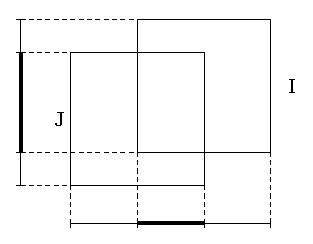
\includegraphics[width=0.25\textwidth]{MA4L4_2.eps}
		\caption{Пересечение брусков $\MI$ и $\MJ$.}
		\label{4_2}
	\end{figure}
	Поскольку у нас пока нет аддитивности, то равенство интегралов будем обосновывать по определению. Пусть оба интеграла существуют. Заметим, что $\MI \cap \MJ$ - замкнутый брус с рёбрами положительной длины, поскольку $A \neq \VN$ и каждая точка $A$ - это внутренняя точка $\MI$ и $\MJ \Rightarrow \MI \cap \MJ$ имеет внутренние точки. Теперь будем строить разбиение. Пусть $\MTB_1$ это разбиение $\MI$, а $\MTB_2$ это разбиение $\MJ$ такие, что на общей части они совпадают. Это можно сделать включением точек концов общих отрезков в разбиение:
	\begin{figure}[H]
		\centering
		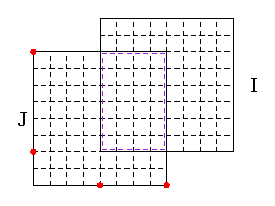
\includegraphics[width=0.25\textwidth]{MA4L4_3.eps}
		\caption{Включение точек концов отрезков пересечения $\MI \cap \MJ$ в разбиение.}
		\label{4_3}
	\end{figure}
	Возьмем отмеченные точки $\xi_1$ для $\MTB_1$ и $\xi_2$ для $\MTB_2$ так, чтобы они совпадали на общей части. Тогда:
	$$
		\sigma(\wte{f},\MTB_1,\xi_1) = \ddsum{j}{}\wte{f}(\xi_j^1){\cdot}|\MI_j^1| = \ddsum{j \colon \MI_j^1 = \MI_j^2}{}\wte{f}(\xi_j^1){\cdot}|\MI_j^1| + \ddsum{j \colon \MI_j^1 \neq \MI_j^2}{}\wte{f}(\xi_j^1){\cdot}|\MI_j^1| = \ddsum{j \colon \MI_j^1 = \MI_j^2}{}\wte{f}(\xi_j^1){\cdot}|\MI_j^1| + 0 =
	$$
	$$
		=	\ddsum{j \colon \MI_j^1 = \MI_j^2}{}\wte{f}(\xi_j^1){\cdot}|\MI_j^1| + \ddsum{j \colon \MI_j^1 \neq \MI_j^2}{}\wte{f}(\xi_j^2){\cdot}|\MI_j^2| = \ddsum{j}{}\wte{f}(\xi_j^2){\cdot}|\MI_j^2| = \sigma(\wte{f},\MTB_2,\xi_2)
	$$
	Разбиваем так, чтобы $\lambda(\MTB_1) \to 0$ и $\lambda(\MTB_2) \to 0$, тогда сразу получаем: $\int_\MI\wte{f}(x)dx = \int_\MJ\wte{f}(x)dx$.
\end{proof}

\begin{defn}
	\uwave{Интеграл Римана по произвольному множеству $A$} (где $A$ - ограничено) это интеграл: 
	$$
		\ddint{A}{} f(x)dx = \ddint{\MI}{} \wte{f}(x)dx, \quad \ovl{A}\subset \Circ{\MI}, \quad
		\wte{f}(x) = 
		\begin{cases}
			f(x), & x \in A \\
			0, & x \not\in A
		\end{cases}
	$$
\end{defn}

\begin{prop}
	$\int_A 1dx$ существует $\Leftrightarrow \partial A$ - множество меры нуль по Лебегу.
\end{prop}
\begin{proof}
	Возьмем $\ovl{A} \subset \Circ{\MI}$, в данном случае $\wte{f}(x) = \chi_A(x)$, тогда по определению:
	$$
		\exists \, \ddint{A}{}1 dx = \ddint{\MI}{}\chi_{A}(x)dx \Leftrightarrow \chi_A(x) \text{ - п.в. непрерывна}
	$$
	Точки разрыва у индикатора могут быть лишь на границе: взяли внутреннюю точку $A \Rightarrow \chi_A \equiv 1$ вместе с некоторой окрестностью, взяли внешнюю точку $\Rightarrow \chi_A \equiv 0$ вместе с некоторой окрестностью $\Rightarrow$ точки разрыва оказываются там, где в окрестности есть точки $A$ и точки дополнения. Если это не так, то либо там есть окрестность, где нет точек $A$ и это внешняя точка, либо там есть окрестность, где нет внешних точек и это внутренняя точка. Во всех остальных случаях мы приходим к граничной точке $\Rightarrow \partial A$ это точки разрыва и $\chi_A(x)$ п.в. непрерывна $\Leftrightarrow \partial  A$ это множество меры нуль по Лебегу. 
\end{proof}

\textbf{Пример}: $A = \MQ \Rightarrow$ граница не является множеством меры нуль по Лебегу.

\textbf{Пример}: $\int_A f(x)dx$ существует, но при этом не существует $\int_A 1 dx$? Да, например: $f(x) = 0$.

\subsection*{Объем допустимого множества}
\begin{defn}
	Множество $A$ \uwave{допустимо} (\uwave{измеримо по Жордану}), если $A$ - ограничено и $\partial A$ это множество меры нуль по Лебегу.
\end{defn}
\begin{defn}
	\uwave{Объемом допустимого множества $A$} (или \uwave{мерой Жордана множества $A$}) называется интеграл: 
	$$
		|A| = \ddint{A}{} 1 dx
	$$
\end{defn}
\begin{rem}
	Заметим, что не нужно путать этот объем с мерой Лебега. Мера Лебега множества рациональных чисел равна нулю, а объем ему приписать нельзя, потому что индикатор этого множества не интегрируем по Риману.
\end{rem}

\begin{prop}
	Если $A$ допустимо и $|A| = 0$, то $\forall$ ограниченная функция $f$ интегрируема по Риману на $A$ и кроме того, верно:
	$$
		\ddint{A}{}f(x)dx = 0
	$$
\end{prop}
\begin{proof}
	Возьмем $\wte{f}(x)$ и брус $\MI \colon \ovl{A} \subset \Circ{\MI}$. $f$ - ограничена $\Rightarrow \wte{f}$ тоже ограничена. Точки разрыва $\subset \ovl{A}$, где $\ovl{A} = A \cup \partial A$, так как вне этого множества функция - тождественный ноль. Поскольку $A$ - допустимо, то $\partial A$ это множество меры нуль по Лебегу и верно:
	$$
		\ddint{\MI}{}\underbrace{\chi_A(x)}_{\geq 0}dx = |A| = 0 \Rightarrow \chi_A(x) = 0 \text{ почти всюду }
	$$
	Поскольку $\chi_A(x) \neq 0$ на множестве $A$, то $A$ это множество меры нуль. Тогда $\ovl{A} = A \cup \partial A$ - множество меры нуль $\Rightarrow$ точки разрыва это множество меры нуль $\Rightarrow \wte{f}$ непрерывана почти всюду и $\wte{f} = 0$ почти всюду, поскольку $A$ это множество меры нуль ($\wte{f} \neq 0$ только на $A$) $\Rightarrow$ интеграл $\int_{\MI} \wte{f}(x)dx$ существует и равен $0 \Rightarrow$ интеграл $\int_{A} f(x)dx$ существует и равен $0$.
\end{proof}
Таким образом, если объем ноль, то это множество меры нуль и любая ограниченаня функция на этом множестве интегрируема.

\begin{theorem}(\textbf{Критерий Лебега для допустимых множеств})
	Пусть $A$ - допустимое множество. Тогда $f$ интегрируема на $A \Leftrightarrow f$ - ограничена на $A$ и непрерывна почти всюду на $A$.
\end{theorem}

\begin{proof}
	$f$ интегрируема на $A \Leftrightarrow \wte{f}$ интегрируема на $\MI \colon \ovl{A} \subset \Circ{\MI} \Leftrightarrow \wte{f}$ - ограничена и почти всюду непрерывна на брусе $\MI$. Следовательно, поскольку $\wte{f}$ ограничена на $A$, то и $f$ ограничена на $A$. 
	
	$\wte{f}$ непрерывна на $\MI \setminus \ovl{A}$, а внутри $A$ она почти всюду непрерывна и там же $\wte{f} = f$. Поскольку $\partial A$ это множество меры нуль $\Rightarrow \wte{f}$ почти всюду непрерывна на $\MI \Rightarrow f$ почти всюду непрерывна на $A$, потому что на $\partial A$ мы не смотрим, а изучаем только внутренние точки. В окрестностях внутренних точек $\wte{f}$ совпадает с $f \Rightarrow \wte{f}$ - ограничена и почти всюду непрерывна на $\MI \Leftrightarrow {f}$ - ограничена и почти всюду непрерывна на $A$. Следовательно, мы получаем требуемое.
\end{proof}
\begin{rem}
	В условии имеется в виду непрерывность почти всюду по $A$ на множестве $A$, но не вообще. То есть проверяются последовательности, которые лежат только в $A$.
\end{rem}
\begin{rem}
	В условии невозможно отказаться от допустимости множества $A$, иначе можно взять функцию Дирихле и множество рациональных чисел $\Rightarrow$ она на нём непрерывна (потому что просто константа), при этом нельзя утверждать, что $f$ интегрируема, так как функция Дирихле не будет интегриурема.
\end{rem}
\begin{rem}
	Если множество не является допустимым, то важной становится сама функция $f$.
\end{rem}

\end{document}